\documentclass[10pt,a4paper]{article}
\usepackage[utf8]{inputenc}
\usepackage{amsmath}
\usepackage{amsfonts}
\usepackage{amssymb}
\usepackage{graphicx}
\usepackage{fancyhdr}
\usepackage{indentfirst}
\usepackage{mathtools}
\usepackage{float}
\usepackage{neuralnetwork}
\setlength{\parindent}{0em}
\setlength{\parskip}{1em}

%\renewcommand{\chaptername}{Course}
\preto{\section}{\clearpageafterfirst}
\preto{\subsection}{\filbreak}
\newcommand{\clearpageafterfirst}{%
  \gdef\clearpageafterfirst{\clearpage}%
}
\newcommand{\yhat}{\hat{y}}
\newcommand{\Yhat}{\hat{Y}}
\newcommand{\lay}[2][]{^{[#2]#1}}
\newcommand{\norm}[1]{\left\lVert#1\right\rVert}

\author{Mohammad Khalaji}
\title{Course 2 - Hyperparameters, Regularization and Optimization}
\begin{document}
\maketitle
% \chapter{Neural Networks and Deep Learning}
\section{Week 1}
\subsection{Train/Dev/Test Sets}
We should always consider the fact that applied ML is an extremely iterative process with many parameters that affect our final outcome. It is virtually impossible to guess those parameters correctly in our first attempt. 
\begin{figure}[h]
    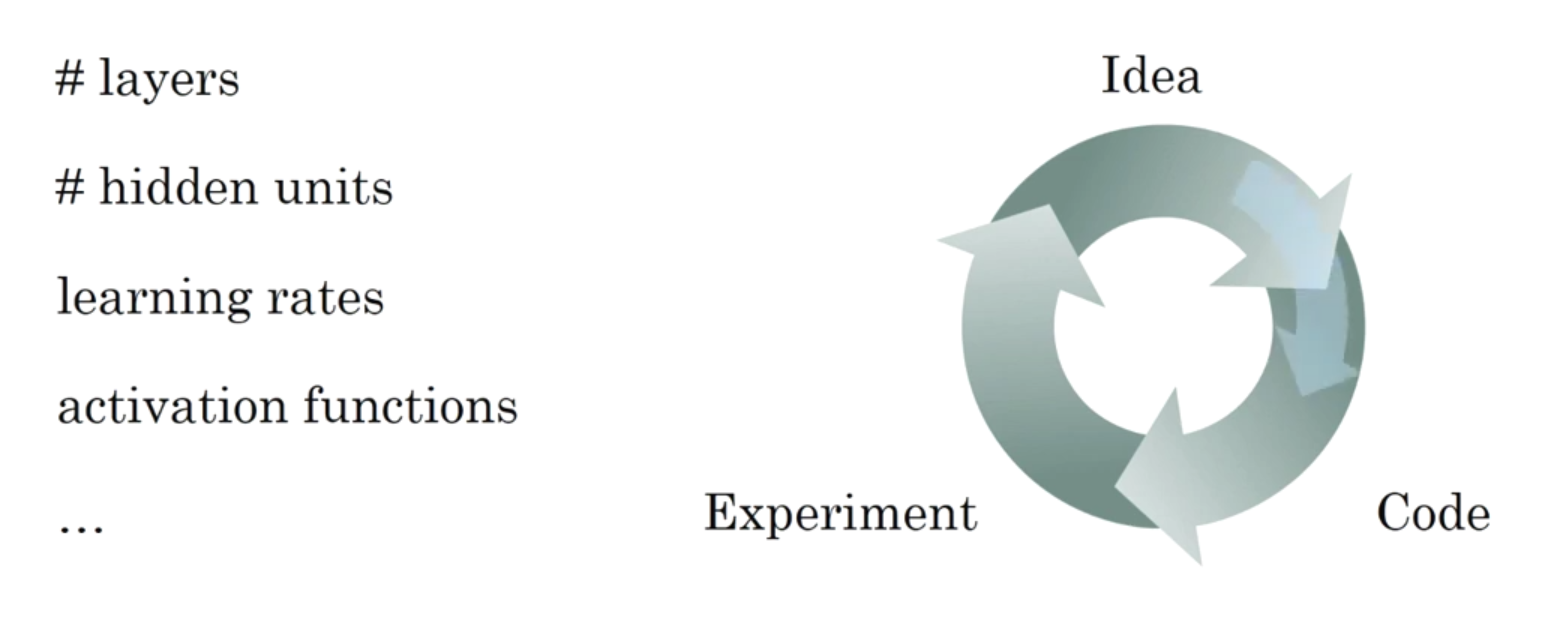
\includegraphics[scale=0.2]{images/iterative.png}
    \centering
\end{figure}

In the previous era of machine learning, it was common to divide all the data and split it according to a 70\%/30\% proportion, and assign them as your train and test sets respectively. Nowadays, however, with the emergence of big data, dev and test sets occcupy a smaller percentage of our data. For example, when we have a dataset with 100000 examples, an 20\% dev set is too big! As a result, the proportions nowadays look like 99.5\%/0.25\%/0.25\%. 

Not having a test set might be okay (only train/dev sets). 


\subsection{Bias/Variance}

The simplest explanation:
\begin{figure}[H]
    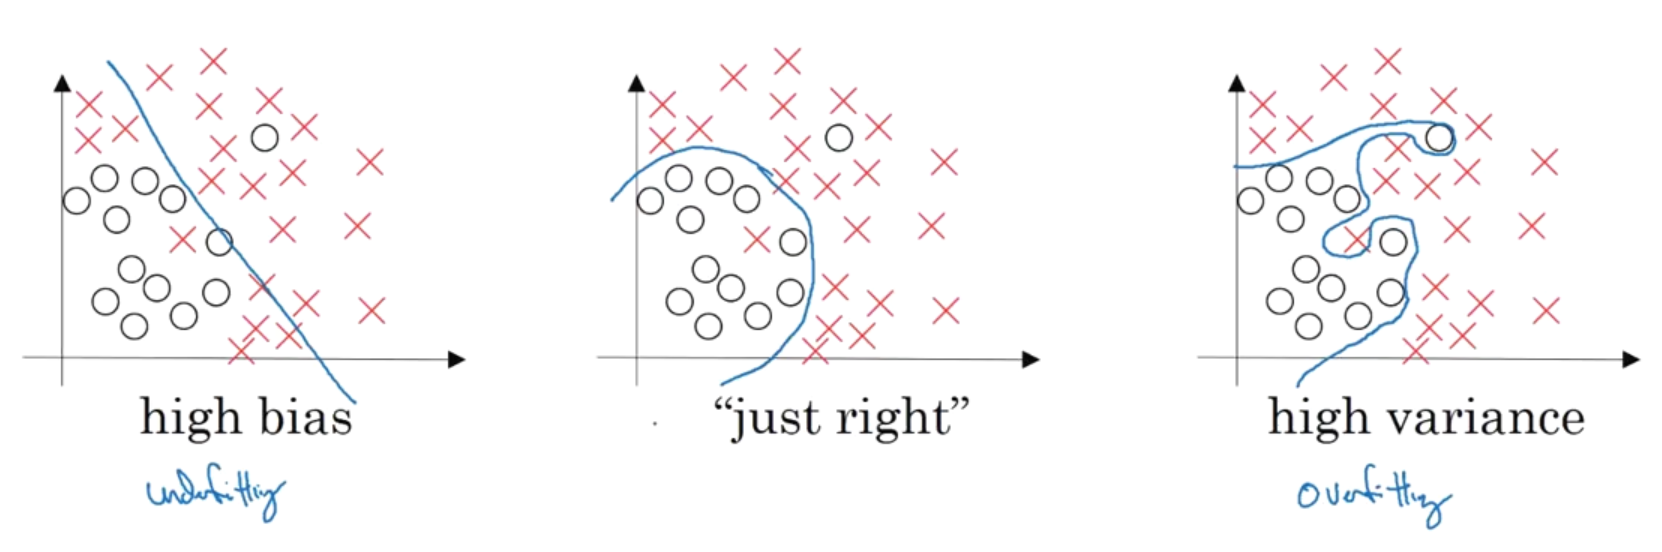
\includegraphics[scale=0.2]{images/biasvariance.png}
    \centering
\end{figure}

Consider another example for a cat classifer. 
\begin{table}[H]
    \begin{tabular}{|c|c|c|c|c|}
    \hline
                & High Variance & High Bias & \begin{tabular}[c]{@{}c@{}}High Bias\\ High Variance\end{tabular} & \begin{tabular}[c]{@{}c@{}}Low Bias\\ Low Variance\end{tabular} \\ \hline
    Train Error & 1\%           & 15\%      & 15\%                                                              & 0.5\%                                                           \\ \hline
    Test Error  & 11\%          & 16\%      & 30\%                                                              & 1.5\%                                                           \\ \hline
    \end{tabular}
\end{table}

The following classifier has both high bias and high variance. High bias because it is a mostly linear classifier, and it mostly underfits; high variance because in some occasions it shows overfitting behavior. 

\begin{figure}[H]
    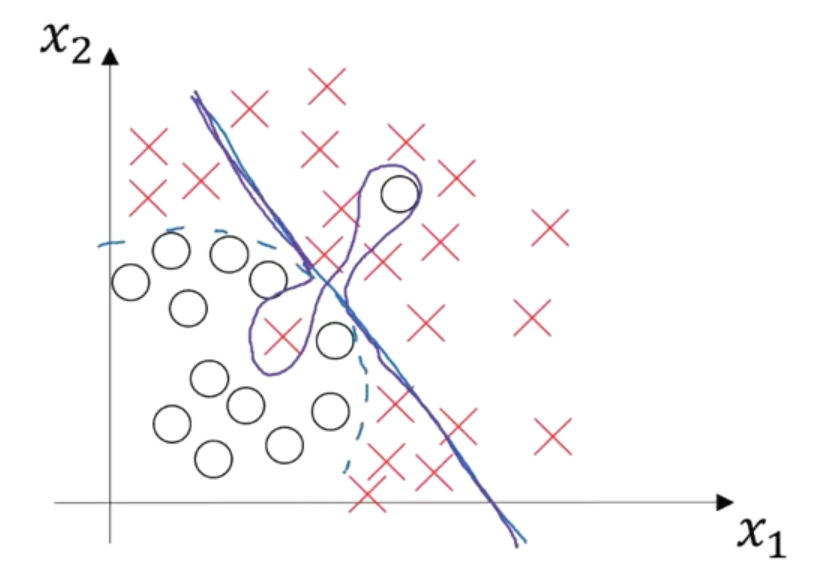
\includegraphics[scale=0.2]{images/highbv.png}
    \centering
\end{figure}

\subsection{Basic Recipe for Machine Learning}
\begin{figure}[H]
    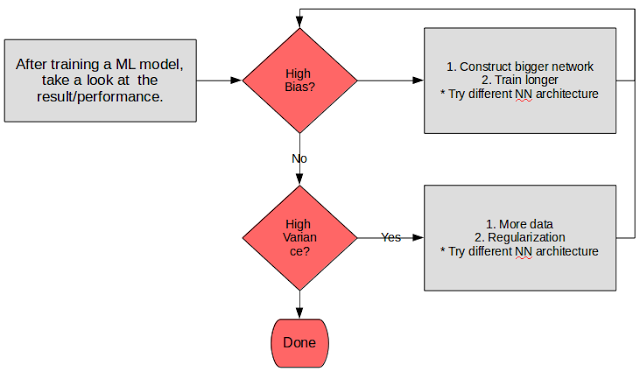
\includegraphics[scale=0.7]{images/recipe.png}
    \centering
\end{figure}

\subsection{Regularization}
If you suspect that your neural network has a high variance problem, meaning that it overfits your data, regularization is one of the first things you should try. The other option is to get more training data, but it is not always viable. 

Remember that in logistic regression, we were trying to minimize $J(w, b)$. Now we add the regularization term to the previous $J$.

$$
J(w, b) = \frac{1}{m}\sum_{i=1}^{m}{L(\yhat^{(i)}, y^{(i)})}+ \frac{\lambda}{2m} \norm{w}_2^{2}
$$ 

It's called $L_2$ regularization because it uses $L_2$ norm, which is: 

$$
\norm{w}_2^2 = \sum_{j=1}^{n_x} w_j^2 = w^T w
$$

It is also possible that we use $L_1$ regularization with the regularization term: 

$$
\frac{\lambda}{2m}\sum_{j=1}^{n_x} |w| = \frac{\lambda}{2m}\norm{w}_1
$$


Note that also a regularization term for bias is possible, but since $b$ is not as high-dimentional as $w$, its regularization term, which is equal to $\frac{\lambda}{m}b^2$, is usually omitted.

In a more complex neural network, though, a more generalized equation will be like this: 

$$
J(W\lay{1}, b\lay{1}, \dots, W\lay{L}, b\lay{L}) = \frac{1}{m}\sum_{i=1}^{m}{L(\yhat^{(i)}, y^{(i)})} + \frac{\lambda}{2m} \sum_{l=1}^L \norm{W\lay{l}}_F^2
$$

$\norm{W\lay{l}}_F^2$ is called the \emph{Frobenius Norm} of the matrix $W\lay{l}$, and knowing that the shape of $W\lay{l}$ is $(n\lay{l-1}, n\lay{l})$ it's computed like this: 

$$
\norm{W\lay{l}}_F^2 = \sum_{i=1}^{n\lay{l-1}} \sum_{j=1}^{n\lay{l}} \Big(w_{ij}^{[l]}\Big)^2
$$

Regularization is also applied to the gradients (it is called \emph{weight decay}): 
$$
dw\lay{l} = (from\ backprop) + \frac{\lambda}{m}w\lay{l}
$$

\subsection{Why Regularization Reduces Overfitting}
Consider a situation where you have a neural network that overfits your data. Remember the original non-regularized cost function: 

$$
J = \frac{1}{m}\sum_{i=1}^{m} L(\yhat^{(i)}, y^{(i)})
$$

In order to reduce overfitting, we penalized $J$ with a regularization term: 
$$
J = \frac{1}{m}\sum_{i=1}^{m} L(\yhat^{(i)}, y^{(i)}) + \frac{\lambda}{2m}\sum_{l=1}^L \norm{W\lay{l}}_F^2
$$

\textbf{Intuition:} If we set $\lambda$ to be a really big number, our minimization algorithm will seek to set $W\lay{l} = 0$, which essentially means that a lot of hidden units will be zeroed out, which means that their impact will be reduced, and we will end up with a simpler neural network that is closer to the "High Bias" realm than it is to the "High Variance" realm.

\textbf{Another Intuition:} Consider using hyperbolic tangent as the activation function. If we regularize our weights, they will become smaller, and as a result, $z = wx+b$ will be smaller. With smaller $z$s, we will be wandering in the "linear section" of $tanh$, which means that each layer will be \emph{roughly} linear, which leaves our network having higher bias. 

\begin{figure}[H]
    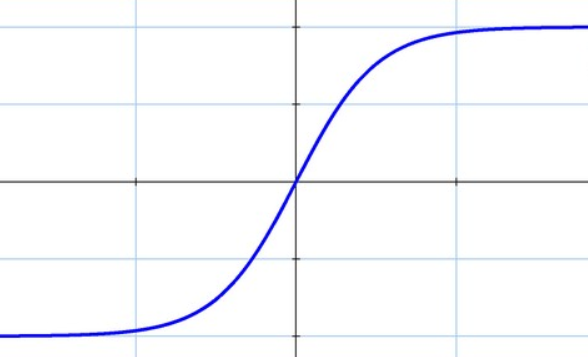
\includegraphics[scale=0.2]{images/tanh.png}
    \centering
\end{figure}
% \newpage
% \section{Week 2}
% \subsection{Mini-Batch Gradient Descent}
We saw how vectorization allows us to perform forward and back propagation easily on $m$ training examples. 

$$
X_{(n_x, m)} = \begin{bmatrix}
    \vline &  & \vline\\
    x\idx{1} & \dots & x\idx{m}\\
    \vline &  & \vline
\end{bmatrix}
$$
$$
Y_{(1, m)} = 
\begin{bmatrix}
    y\idx{1} & \dots & y\idx{m}
\end{bmatrix} 
$$

What if $m=5000000$? We split our training set into mini batches of, say $1000$ training samples.
$$
X\ Batches: X\batch{1}, \dots, X\batch{5000}
$$ 
$$
Y\ Batches: Y\batch{1}, \dots, Y\batch{5000}
$$

\begin{itemize}
    \item for $t=1\dots5000$ do:
    \begin{itemize}
        \item[-] Forward Prop on $X\batch{t}$
        \begin{itemize}
            \item[] $Z\lay{1} = W\lay{1}X\batch{t}+b\lay{1}$
            \item[] $A\lay{1} = g\lay{1}(Z\lay{1})$ 
            \item[] $\dots$
            \item[] $Z\lay{L} = W\lay{L}A\lay{L-1}+b\lay{L}$
            \item[] $A\lay{L} = g\lay{L}(Z\lay{L})$ 
        \end{itemize} 
        \item[-] Compute Cost: $J\batch{t}=\frac{1}{1000}\sum{\dots} + \dots$
        \item[-] Back Prop to compute gradients with respect to $J\batch{t}$. 
        \item[-] Update parameters.   
    \end{itemize}
\end{itemize}

\subsection{Understanding Mini-Batch Gradient Descent}

\begin{figure}[H]
    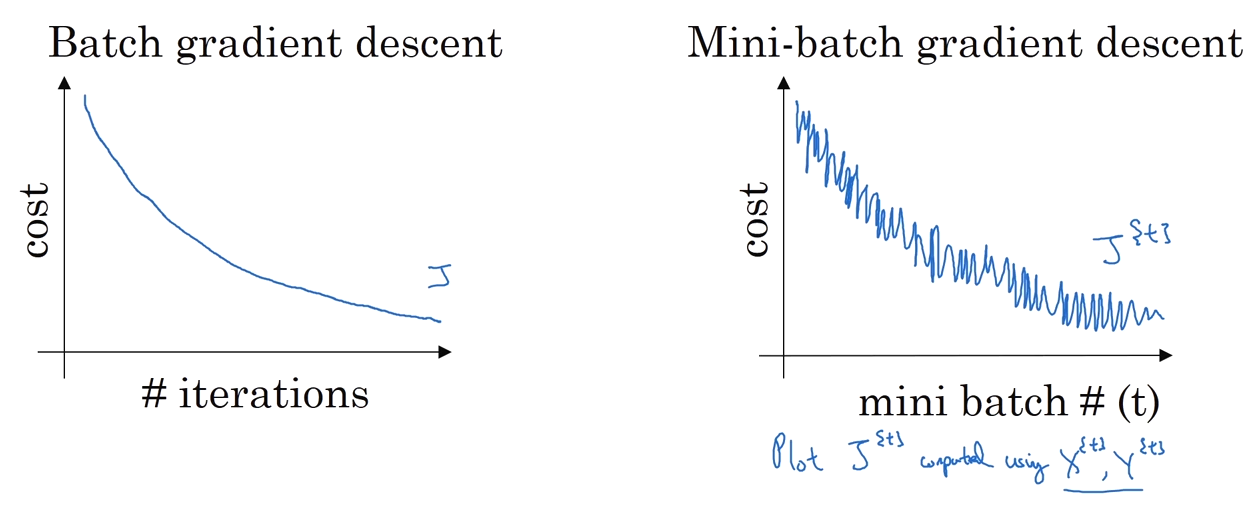
\includegraphics[scale=0.35]{images/minibatch.png}
    \centering
\end{figure}

\begin{itemize}
    \item If mini-batch size equals $m$: Batch Gradient Descent (Blue)
    \item If mini-batch size equals $1$: Stochastic Gradient Descent (Purple)
\end{itemize}

\begin{figure}[H]
    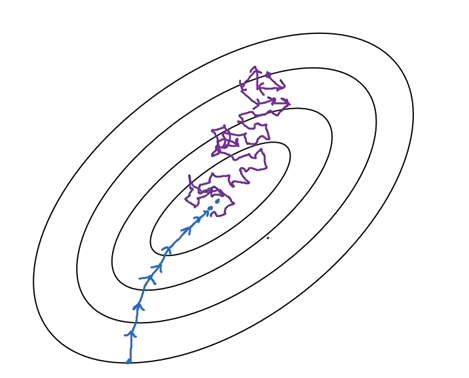
\includegraphics[scale=0.35]{images/stochastic.png}
    \centering
\end{figure}

\textbf{Batch Gradient Descent:} Too long per epoch.

\textbf{Stochastic Gradient Descent:} Losing the speed-up of vectorization. 

\textbf{Somewhere in Between:} Take advantage of the speed-up of vectorization + Make progress without needing to wait. Typical mini-batch sizes are $64, 128, 256, 512$. Make sure your mini-batches fit in CPU/GPU memory. 


% \newpage
% \section{Week 3}
% \subsection{Tuning Process}
Tuning hyperparameters: 
\begin{itemize}
    \item First in importance: $\alpha$
    \item Second in importance: $\beta$, no. of hidden units, mini-batch size
    \item Third in importance: no. of layers, learning rate decay
\end{itemize}

While using the Adam optimization algorithm, it is almost never necessary to tune $\beta_1, \beta_2, \epsilon$ since the default values are pretty decent.

People usually advise against using a grid for tuning hyper parameters, since for each hyperparameter, a limited number of values is tried, and if one of the hyperparameters is of less importance, a lot of tries will be useless. 
\begin{figure}[H]
    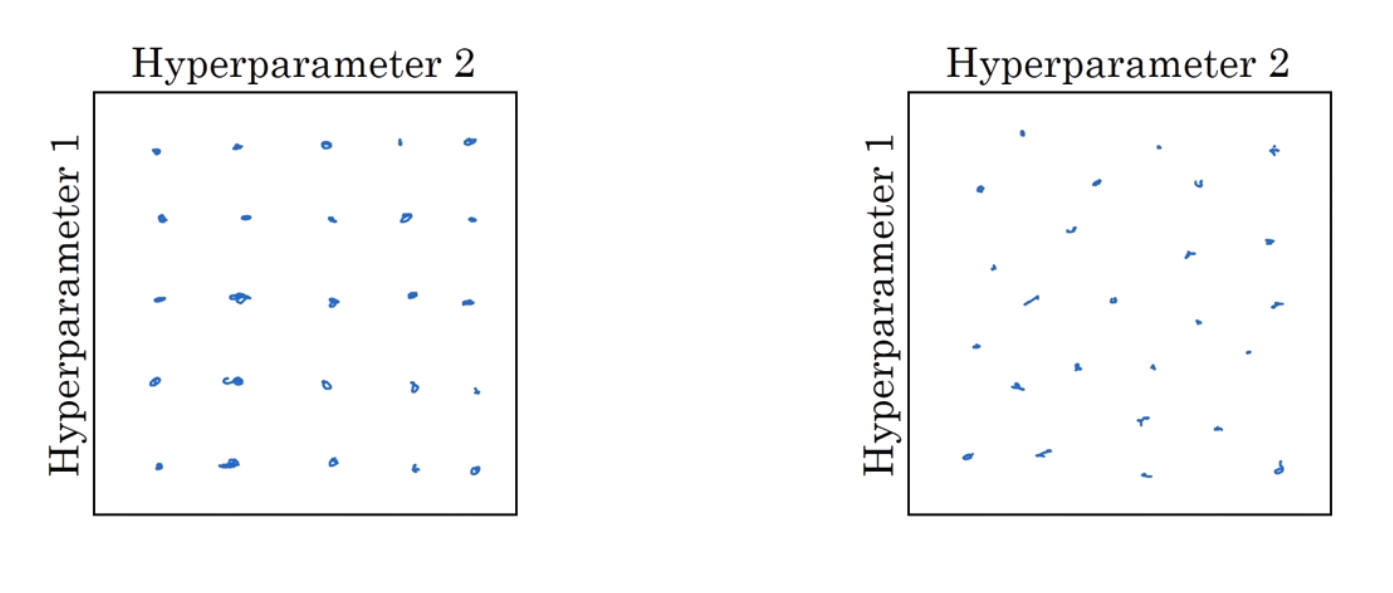
\includegraphics[scale=0.25]{images/hyp.png}
    \centering
\end{figure}

\textbf{Coarse to Fine Approach}: 
\begin{itemize}
    \item Sample random points in hyperparameters space
    \item Choose the points with the best performance
    \item Zoom in inside the space where those points reside
    \item The new hyperparameter space is the zoomed-in region
    \item Repeat
\end{itemize}

\subsection{Using an Appropriate Scale}
Random sampling is not enough. Consider a situation where you want to choose $n\lay{l}$ for a given layer, and you think that values between $50$ and $100$ are appropriate. 
In the $[50, 100]$ interval, it is pretty reasonable to choose some values randomly. 
Same goes for $L$. even a grid search might be reasonable. 

However, this is not true for all hyperparameters. As an example, imagine that you are trying to choose an appropriate $\alpha$ in the range $[0.0001, 1]$.
If you choose some values randomly, $90\%$ of the values will be greater than $0.1$, and only $10\%$ will be in the interval $[0.0001, 0.1]$, which typically contains desirable values. 
The solution is to choose a logarithmic scale. 
Use $[-4, 0]$ to choose a random value $r$, and set $\alpha=10^{r}$. 

\textbf{Hyperparameters for Exponentially Weighted Averages:} 

Remember that $\beta=0.9$ basically meant that we were taking the average of last $10$ values, whereas $\beta=0.999$ was as if we were taking the average of the last $1000$ values. 
As a result, using a linear scale for generating random $\beta$ is not suitable. 
The solution is to randomly find a suitable $1-\beta$ using the logarithmic scale mentioned above. 
$$
1-\beta = 0.001 \dots 0.1
$$

\subsection{Hyperparameter Tuning in Practice}
\begin{itemize}
    \item Re-test hyperparameters occasionally. Re-evaluate once every several months.
    \item Use hyperparameters that other researchers have used. 
\end{itemize}

Too major schools of thought when it comes to hyperparameter tuning: 
\begin{enumerate}
    \item The panda approach: Babysitting one model: usually on huge datasets, weak computational resources. When you only afford to train one model. For example, change the learning rate everyday in the middle of training process. 
    \item The caviar approach: Training many models in parallel
\end{enumerate}

\subsection{Normalizing Activations in a Network}
The algorithm is called Batch Normalization. It makes your hyperparameter search easier, and it enables you to train very deep networks.

We learnt to normalize the inputs: 
$$
\mu = \frac{1}{m}\sum_{i=1}^{m} x\idx{i}
$$
$$
X = X-\mu
$$
$$
\sigma^2 = \frac{1}{m}\sum_{i=1}^{m} x^{(i)^2}
$$
$$
X = \frac{X}{\sigma^2}
$$

However, in deep models, not only do we have input units, we also have many hidden units (activations). 
For example, normalizing the values of $a\lay{2}$ might help us train $W\lay{3}, b\lay{3}$ more efficiently.


The question: Can we normalize the values of $a\lay{l-1}$ so as to train $W\lay{l}, b\lay{l}$ faster?

Technically, in batch normalization we do not normalize the values of $a\lay{l-1}$, but we DO normalize the values of $z\lay{l-1}$. 
In practice, normalizing $z$ is used much more often. 

Given some $Z$ in some layer: 
$$
Z = \begin{bmatrix}
    \vline & & \vline\\
    z\idx{1} & \dots & z\idx{m}\\
    \vline & & \vline
\end{bmatrix}
$$
(the square brackets corresponding to the layer are omitted here)
$$
\mu = \frac{1}{m}\sum_{i=1}^{m} z\idx{i}
$$

$$
\sigma^2= \frac{1}{m}\sum_{i=1}^{m} (z\idx{i} - \mu)^2
$$
$$
z\idx{i}_{norm} = \frac{z\idx{i} - \mu}{\sqrt{\sigma^2 + \epsilon}}
$$

Result: Every $z$ component will have a $0$ mean and a $1$ standard deviation. 
But we do not want this! What we do instead: 
$$
\tilde{z}^{(i)} = \gamma z\idx{i}_{norm} + \beta
$$
Where $\gamma, \beta$ are learnable parameters, which means that they are updated like weights and biases.

Special case: 
$$
\gamma = \sqrt{\sigma^2 + \epsilon}, \beta = \mu
$$
$$
\Rightarrow \tilde{z}^{(i)} = z\idx{i}
$$
We will use $\tilde{z}^{(i)}$ instead of $z\idx{i}$ for the latest computation. 


\subsection{Fitting Batch Norm into Neural Networks}
$$
X \xrightarrow{W\lay{1}, b\lay{1}} Z\lay{1} \xrightarrow{\gamma\lay{1}, \beta\lay{1}} \tilde{Z}\lay{1} \xrightarrow{g\lay{1}} A\lay{1} = g\lay{1}(\tilde{Z}\lay{1}) \rightarrow \dots
$$
As a result, we have new parameters $\beta\lay{l}, \gamma\lay{l}$ for each layer. 

\textbf{Important:}

We saw that: 
$$
Z\lay{l} = W\lay{l}a\lay{l-1} + b\lay{l}
$$
And we know that batch norm will first compute $Z_{norm}$, which means that $Z$'s mean will be subtracted form it.
As a result, adding a constant like $b\lay{l}$ while computing $Z\lay{l}$ does not do anything because any constant that we add, is going to be cancelled out by the batch norm step.

So, when using batch norm, biases can be simply eliminated from our parameters. 

Needless to say, both $\gamma\lay{l}$ and $\beta\lay{l}$ are of shape $(n\lay{l}, 1)$. 

\begin{itemize}
    \item for $t=1 \dots No.\ of\ MiniBatches$
    \begin{itemize}
        \item[] Forward Prop on $X\batch{t}$ 
        \item[] In each hidden layer, use batch norm to replace $Z\lay{1}$ with $\tilde{Z}\lay{1}$. 
        \item[] Use Back Prop to update the parameters $W\lay{1} \dots W\lay{L}$, $\gamma\lay{1} \dots \gamma\lay{L}$, $\beta\lay{1} \dots \beta\lay{L}$. (NO BIASES) 
    \end{itemize}
\end{itemize}

\subsection{Why Does Batch Norm Work?}
Batch norm is doing a similar thing to normalizing our input data. 

Moreover, when our data becomes subject to Covariate Shift, a non-batch-normalized network might not do very well. Example: Black vs. Colored cats classifier. 
It helps the hidden layers be more stable. 

It also has a slight regularization effect. 

\subsection{Batch Norm at Test Time}
Batch norm is dealing with batches in train time. However, it deals with single data points in test time. 
Recall the equations of batch norm: 
$$
\mu = \frac{1}{m}\sum_{i=1}^{m} z\idx{i}
$$
$$
\sigma^2= \frac{1}{m}\sum_{i=1}^{m} (z\idx{i} - \mu)^2
$$
$$
z\idx{i}_{norm} = \frac{z\idx{i} - \mu}{\sqrt{\sigma^2 + \epsilon}}
$$
$$
\tilde{z}^{(i)} = \gamma z\idx{i}_{norm} + \beta
$$

We must have a different way of coming up with a $\mu$ and $\sigma^2$ because taking the mean and the variance of one example does not make sense. 

\textbf{Solution:} Estimate $\mu$ and $\sigma^2$ using exponentially weighted averages across mini batches. 
In each batch, we have $L$ different values for $\mu$ and $\sigma^2$ corresponding to different layers $\rightarrow$ Take their exponentially weighted average!

\subsection{Softmax Regression}
Classifiers that classify data and assign them to one of more than only 2 classes use softmax regression. 

If we have $C$ classes, we must have a neural network whose output layer has $C$ units. For example: $C=4$: 


\begin{neuralnetwork}[]
    \newcommand{\x}[2]{$x_#2$}
    \newcommand{\y}[2]{$z\lay{L}_#2$}
    \newcommand{\hfirst}[2]{\small $\ $}
    \newcommand{\hsecond}[2]{\small $\ $}
    \newcommand{\hthird}[2]{\small $\ $}
    \newcommand{\hfourth}[2]{\small $\ $}

    \inputlayer[count=4, bias=false, title=, text=\x]
    \hiddenlayer[count=5, bias=false, title=, text=\hfirst] \linklayers
    \hiddenlayer[count=5, bias=false, title=, text=\hsecond] \linklayers
    \hiddenlayer[count=4, bias=false, title=, text=\hthird] \linklayers
    \outputlayer[count=4, title=, text=\y] \linklayers
\end{neuralnetwork}

We know that: 

$$
z\lay{L} = W\lay{L}a\lay{L-1} + b\lay{L}
$$
Activation function: 
$$
temp = e^{(z\lay{L})}
$$
As we know, the shape of both $z\lay{L}$ and $temp$ is $(4, 1)$.  
$$
a\lay{L} = \frac{e^{(z\lay{L})}}{\sum_{i=1}^{4} temp_i}
$$

\subsection{Training a Softmax Classifier}
Softmax regression generalizes logistic regression to $C$ classes. 

\textbf{Loss Function:}

$$
L(\yhat, y) = -\sum_{j=1}^{C} y_j log(\yhat_j)
$$

\end{document}